\section{An Illustrative Example} 
\label{sec:example}

We define a simple autonomous underwater vehicle (AUV) mission that will be used to illustrate the
benefits of our approach compared to previous ones and the major
issues that arise when dispatching. First, the AUV can be at a
location or be traveling to one. Second, the AUV has a few basic
actions that allow it to function within the environment.  It can go
to a location, survey a location, and sample a location. In a typical
AUV mission, the scientist will want it to survey and sample a
location and, if needed, be redirected on the fly to a new location for
surveying and surveying.

\begin{figure}[!htb]
  \centering
  \subfloat[\small Bathymetry of vent sites off of NW United States]{\label{fig:ex:axial}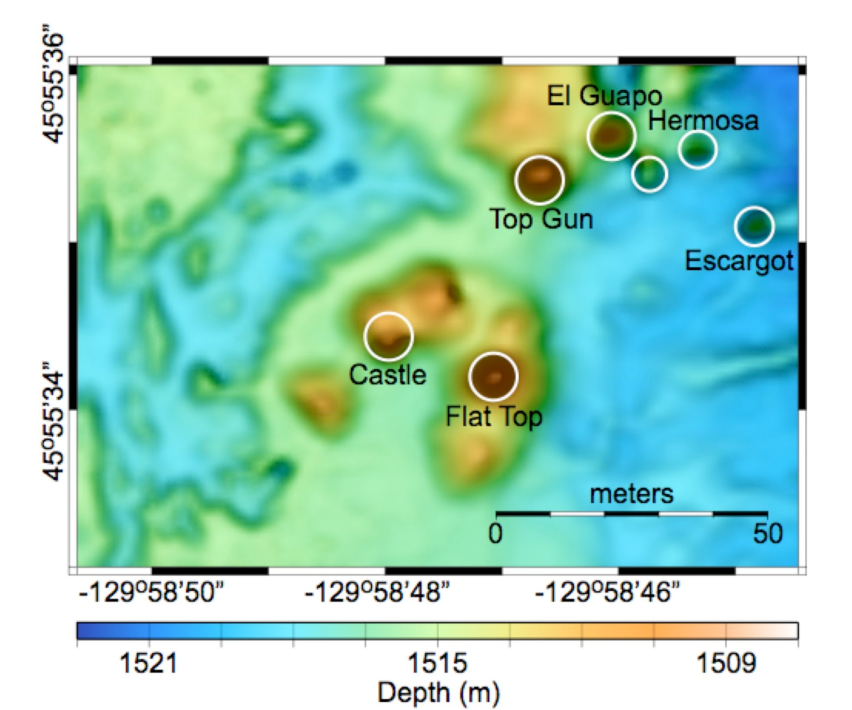
\includegraphics[scale=0.35]{figs/vents.pdf}}\\
  \subfloat[\small An illustration of our domain]{\label{fig:ex:graph}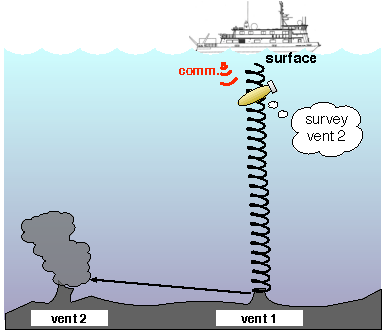
\includegraphics[width=0.51\columnwidth]{figs/auv_example}}
  \hfill \subfloat[\small Initial  problem]{\label{fig:ex:init}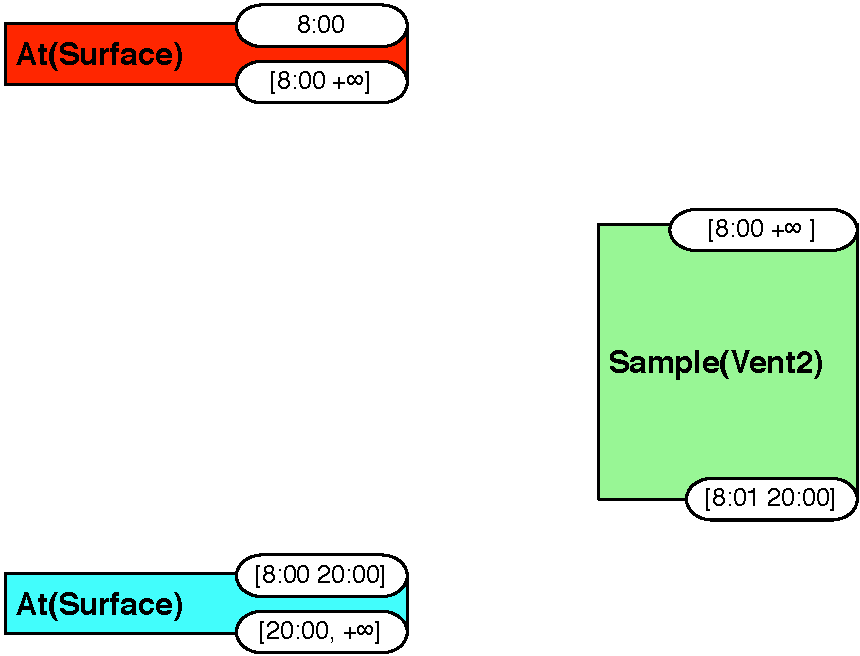
\includegraphics[width=0.47\columnwidth]{figs/example_initial}}
  \caption{\small{\ref{fig:ex:axial} shows bathymetry of actual vent
      sites off the coast of Oregon. A description of a hydrothermal
      vent problem with an illustration of the domain
      (\ref{fig:ex:graph}) along with the initial partial plan for
      this problem (\ref{fig:ex:init}). In this domain our AUV is
      initially at {\em Surface} at 8am, he wants to survey {\em vent
        2} and needs to be back at {\em
        Surface} before the end of its mission at 8pm (noted 20:00
      here).}}
\label{fig:Example}
\end{figure}

However, an issue with finding a balanced approach is deciding whether
to start an action as early as possible --- which we will call {\em
proactive} --- or wait until the action should necessary start ---
called later {\em deferred}.  There is a clear difference between the
two approaches but when should, for example, the AUV wait or start
early? We demonstrate a scenario where the AUV ideally uses the two
approaches at different times. The initial problem is illustrated in Figure
\ref{fig:Example}.

The AUV mission starting at 8 AM needs to {\em sample vent2} and
return to the {\em ship} by 8 PM. The AUV starts traveling immediately
to {\em vent1}. Considering that that it takes one to two hours to go
from the {\em Surface} to {\em vent1}, roughly ten minutes to go from
{\em vent1} to {\em vent2}, and more than two hours in order to {\em
survey} and {\em sample}, a general plan solution is presented in
Figure \ref{fig:ex:plan}. The plan presented here is partially
instantiated giving the AUV the freedom to decide {\em when} to start
each action within the valid boundary of the solution. For example,
the AUV should go early in order to {\em sample vent2} so that the
scientists have the a possibility for requesting more
tasks. Conversely, heading back to the surface early would waste
valuable time, roughly two hours, if the scientists decide they want to
{\em survey} another location. Though by 6pm, it should go to the
surface so the scientists can pick it up by 8pm. In this scenario, we
see that the AUV alternated between deciding to execute actions early
or {\em defer} them depending on the nature of the action it needed to
take next, or more accurately the nature of the objectives related to
this action. The AUV was {\em proactive} on traveling to {\em sample vent2}
because the scientists want it to be completed. On the other hand, the
AUV has to return to the surface by 8 PM, however, the scientists don't
explicitly want this done, allowing it to procrastinate.  By
doing so, the AUV is available to complete new tasks given to it by
the scientist.\fcomment{One concept that would help if introduced is
  around the same notion of task span in plan optimization : we have
  the same problem here but we use a more refined execution policy in
  order to avoid extraneous actions should a goal come back to us.}

% \fcomment{Need a figure that shows the plan somehow ... this can be
%   refined as we go along for illustrating proactive vs deferred}

\begin{figure}[!htb]
  \centering
  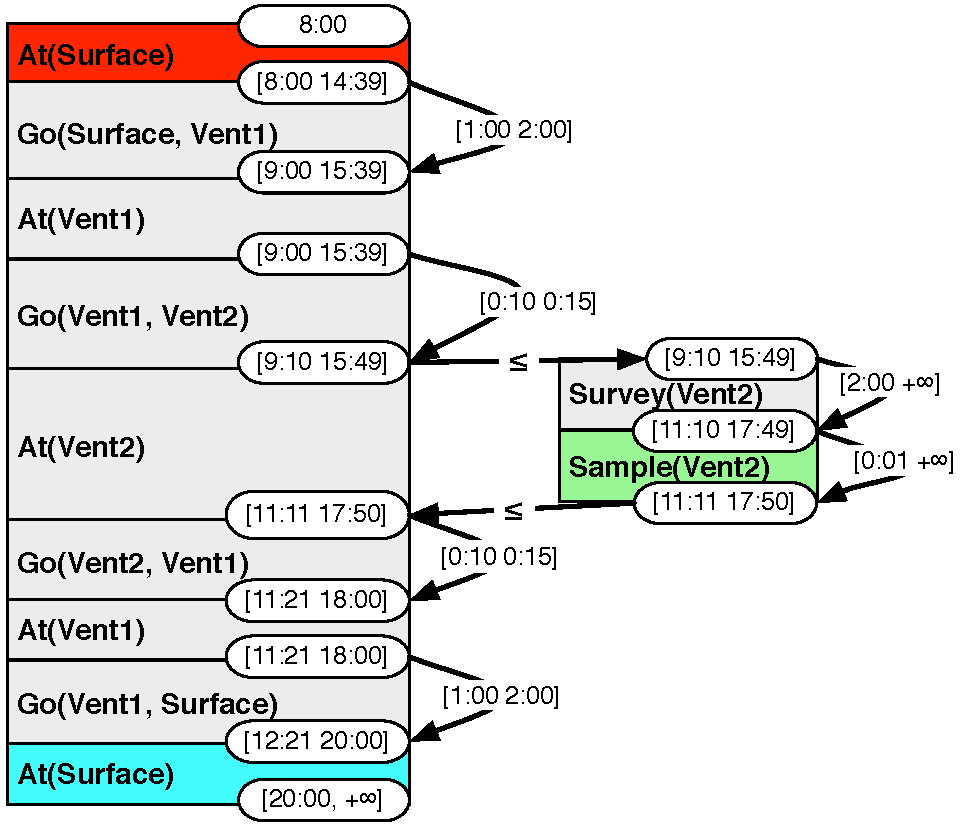
\includegraphics[width=0.8\columnwidth]{figs/example_plan}
  \caption{The flexible plan solution of our domain in
    Fig. \ref{fig:Example}}
  \label{fig:ex:plan}
\end{figure}

While this example may appear academic at first, it reflects situations
we have seen within embedded agent execution in our domain. Indeed, we
do daily operations wehere our AUV is deployed and scientists can
remotely send new objectives as the mission goes along to the vehicle
as they see new areas of interest. Especially in the upper water
column the nature of the area to be examined depends highly on the
dynamic of the ocean itself and is difficult to predict beforehand. Therefore,
scientist can use data sampled by the AUV or other sources (eg
satellite data, ship based observations, \dots{}) during the beginning of
the operation in order to give it better informed objectives for the
rest of the operation. At the same time the vehicle has
also operational objectives such as going to a place where its
recovery will be easier for operators. This gives a similar
distinction between the science objectives and operation
objectives. Similarly to our example we do not really want the
AUV to get back to recovery area too early as a new science goal could
be sent to it which in turn would rather be fulfilled as early as
possible.

This paper discusses the problem of dispatching when trying to execute
a plan. In particular, dispatching in a dynamic environment where the
plan is expected to change due either to unanticipated events or external
requests with new directives. External requests  can occur
at any time which make them in essence uncontrollable events.
Specifically, we focus on how these new requests, coming from the
external world, alter the way we need to dispatch the plan, rather than
how they will be integrated into the plan or any part of the planning
process. The reason for our separation from planning is that
oftentimes planning and executing are split up into two different
jobs. Often times a robotic agent is given an already created plan, and it
must then choose when to execute parts of the plan. Therefore, our focus is on
developing a method for dispatch a plan, after it has already been created, while
understanding that new requests may come in the future.

The approach we have taken on dispatching looks at the token level of a plan,
specifically at tokens generated from external requests which we define as goals.
Because they have been requested by an external person with the intent of being 
completed promptly, they have a high priority. In contrast, there are tokens that only describe the
evolution of a timeline, which we define as non-goals. In order to keep the plan 
valid, the agent is obligated to complete the non-goals, but there is no rush. Thus, the
non-goals have a low priority. Therefore, we want to complete the goals
as early as possible in order to give adequate time for the possibility of new
goals, and complete the non-goals as they become necessary for the validity of the plan. 
Some may argue that finishing the goals early doesn't guarantee that
there will be enough time for new goals, however, that is an issue with planning, 
and our concern is whether dispatching caused the waste of time.


%%% Local Variables: 
%%% mode: latex
%%% TeX-master: "aaai13"
%%% End: 
